\section{Evidence base I: direct attacks on language models}\label{sec:evidence}

\subsection{Three structural facts}

The 2023--2026 record on direct jailbreaks supports three structural facts, and the
third is the one that changes engineering plans.

\textbf{Fact 1: the optimization frontier is fully broken.} Every frontier model
tested by adversarial-optimization research has been jailbroken: gradient-based
GCG suffixes transfer across aligned models \cite{gcg}; automated red-team loops
reach tens of queries with high success on black-box access \cite{pair,tap}; and
in-the-wild jailbreak mining (WildTeaming) harvested thousands of compositional
attack paths from real chat logs \cite{wildteaming}. The correct planning
assumption is not ``model $X$ is safe'' but ``single-turn policy text is a
speed bump''.

\textbf{Fact 2: static defenses fail against adaptive attackers.} Whatever the
guard---input classifiers, output filters, refusal training---published
adaptive evaluations keep finding bypasses, because the attacker iterates on the
defender's responses while the defense is fixed at deploy time. This is the core
argument for our self-probe plane (Section~\ref{sec:gaps}): a guard's honest score
is its score \emph{under escalation}, which is what a one-shot suite never
measures. Guard wear is a measurable phenomenon, not a rhetorical one.

\textbf{Fact 3: the automation cost collapsed.} PAIR reached compliance with
fewer than twenty black-box queries and roughly three cents of API spend
\cite{pair}; TAP pruned the search with a tree and a judge \cite{tap}; RedAgent
brought context-aware attack generation to five-query budgets on agent stacks
\cite{redagent}. When the marginal cost of an attack attempt rounds to zero,
\emph{frequency} becomes the attacker's weapon and the defender's statistics must
be expressed per-session, not per-attempt---this motivates the retry-inflation
machinery of Section~\ref{sec:stats}.

\subsection{Attack-success rates: the anchor table}\label{sec:asr}

Table~\ref{tab:asr} collects the published attack-success anchors this paper's
priors rest on. Two warnings before reading it. Heterogeneity is real: targets,
judges, and guard regimes differ, which is why we pool with per-study posteriors
(Section~\ref{sec:pooling}) rather than merging counts. And several rows are
LLM-judged; judge dependence is carried as its own class (W8).

\begin{longtable}{L{3.4cm} L{2.8cm} L{1.7cm} L{1.3cm} L{2.6cm}}
\caption{Published ASR anchors (undefended arm unless noted). ``judge'' marks
rates decided by an LLM judge.}\label{tab:asr}\\
\toprule
Study / benchmark & Attack family & Reported ASR & Arm & Notes \\
\midrule
\endfirsthead
\toprule
Study / benchmark & Attack family & Reported ASR & Arm & Notes \\
\midrule
\endhead
\bottomrule
\endfoot
GCG \cite{gcg} & gradient suffix, transfer & $\sim$60\% & undef. &
transfer across aligned models \\
PAIR \cite{pair} & automated social eng. & $\sim$43\% median; $<$20 queries &
undef. & judge-dependent \\
TAP \cite{tap} & tree-of-attacks w/ judge & high on evaluated models &
undef. & pruned by judge \\
WildTeaming \cite{wildteaming} & mined multi-turn & 4.6$\times$ diverse paths &
undef. & mining, not ASR \\
InjecAgent \cite{injecagent} & direct-tool injection & 34\% direct; 59\%
directive & undef. & tool-integrated \\
AgentDojo \cite{agentdojo} & indirect injection suite & 34.5\% & undef. &
real-task env \\
AgentDojo + CaMeL \cite{camel} & same suite, capability lattice & 6.8--8.0\% &
\textbf{def.} & utility cost discussed \\
PoisonedRAG \cite{poisonedrag} & 5 poisoned docs into corpus & 90\% & undef. &
RAG corruption \\
AgentPoison \cite{agentpoison} & $<$0.1\% poisoned memory rows & $>$80\% &
undef. & persistent backdoor \\
AgentHarm \cite{agentharm} & overtly harmful agent tasks & 34.7\% & undef. &
misuse compliance \\
SafeArena \cite{safearena} & harmful web-agent tasks & high compliance
across agents & undef. & web-agent plane \\
SafeAgentBench \cite{safeagentbench} & embodied unsafe planning & 10\%
refusal-aware & undef. & embodied plane \\
tau-bench \cite{taubench} & pass$^8$ reliability & $<$25\% & n/a &
reliability, not attack \\
Language Barrier \cite{langbarrier} & multilingual safety gap & 79\% vs 80.9\%
harm-enabling & undef. & EN vs low-resource \\
One Jailbreak, Many Tongues \cite{onetongue} & language-insensitive reps &
transfer across langs & undef. & 2026 preprint \\
Low-resource jailbreak \cite{lowresjb} & low-resource probes & guardrail drop
9--18 pts & undef. & 2026 preprint \\
\end{longtable}

The two pools this paper's priors use summarize this table: pooling the
undefended rows gives a Beta--Binomial posterior mean of 0.296 (sd 0.010), the
defended rows 0.075 (sd 0.007)---defenses cut the pooled success rate by
${\sim}3.96\times$ while leaving a material residual (Section~\ref{sec:pooling}).
Figure~\ref{fig:asr} plots the anchor rates; hollow bars mark the defended arm.

\begin{figure}[htbp]
\centering
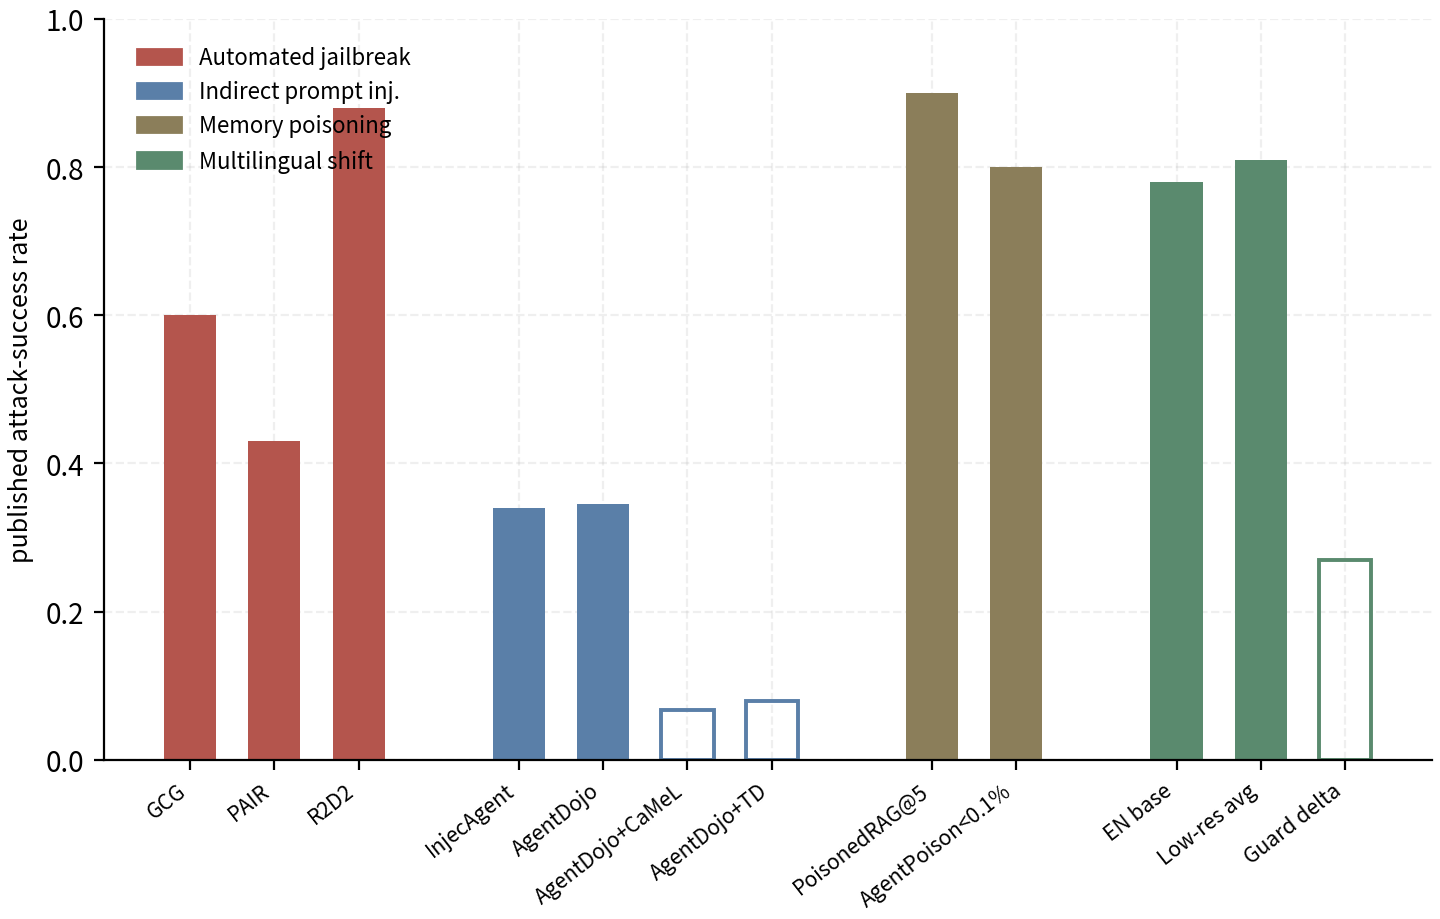
\includegraphics[width=0.98\columnwidth]{fig_asr.png}
\caption{Published attack-success anchors by family (Table~\ref{tab:asr}).
Hollow bars = defended arm: the defended residuals (CaMeL 6.8--8.0\%) are the
planning numbers---low, material, and priced in utility.}\label{fig:asr}
\end{figure}

\subsection{Multilingual erosion (W13)}\label{sec:multilingual}

The multilingual evidence is unusually consistent: harm-enabling compliance
rates around 79\% in English rise to ${\sim}80.9\%$ averaged over low-resource
languages \cite{langbarrier}, guardrails measured in English lose 9--18 points
under low-resource probes \cite{lowresjb}, and 2026 mechanistic work shows
language-insensitive intention representations carrying jailbreaks across
languages once one is learned \cite{onetongue}. For an English-first framework
the implication is uncomfortable: our probes, our guard text, and our judges are
all English, so our measured robustness is the \emph{best} case of a
distribution we do not sample. The multilingual probe pack in our self-probe
arsenal exists to make that blind spot measurable (Section~\ref{sec:gaps}).

\subsection{What this means for orchestration frameworks}

Two implications are specific to frameworks like ours. First, the same
orchestration machinery that makes probing cheap makes target-side defense cheap:
a framework can resample, retry, and escalate---which is exactly why its
\emph{reported} success rates need the resampling-null discipline of
Section~\ref{sec:stats} (a raw-retry harness measures its own patience). Second,
the framework is on the receiving end of everything in this table: its planner is
prompt-injectable through fetched content (W1), its memory is poisonable (W5),
and its guard chain is jailbreakable by construction (W2). The honest posture is
to run this table's attacks against ourselves as a scheduled control, not to
assume good intentions from our own code.
